% igs2eguide.tex
% v2.00 12-jun-08

\NeedsTeXFormat{LaTeX2e}

% The default is for Journal of Glaciology, one column, A4 paper. The other options are listed below:

%\documentclass{igs}
%\documentclass[twocolumn]{igs}
% \documentclass[annals]{igs}
% \documentclass[annals,twocolumn]{igs}

%\documentclass[letterpaper]{igs}
%\documentclass[twocolumn,letterpaper]{igs}
% \documentclass[annals,letterpaper]{igs}
% \documentclass[annals,twocolumn,letterpaper]{igs}

% when submitting your article for review, use one
% of the following two options:

\documentclass[review]{igs}
% \documentclass[annals,review]{igs}

\usepackage{igsnatbib}
\usepackage{stfloats}
\usepackage{graphicx}
\usepackage[english]{babel}        % language english

% the default is for unnumbered section heads
% if you really must have numbered sections, remove
% the % from the beginning of the following command
% and insert the level of sections you wish to be
% numbered (up to 4):

% \setcounter{secnumdepth}{2}

%\newcommand{\BSecular}{-65$\pm$15 Gt a$^{-1}$}
%\newcommand{\BSecularAvgSeas}{-71$\pm$15 Gt a$^{-1}$}

\begin{document}

\title[GRACE Forward Modeling]{GRACE forward modeling of Gulf of Alaska water balances}

\author[Arendt and others]{Authorship TBD}

%\affiliation{%
%$^1$Applied Physics Laboratory, University of Washington \\ E-mail: arendta@uw.edu \\ $^2$Planetary Geodynamics Laboratory, NASA Goddard Space Flight Center, Code 698, Greenbelt, MD, 20771\\ $^3$ School of Civil and Construction Engineering, Oregon State University, Corvallis, OR, 97331, USA}

\abstract{.}

\maketitle

\section{Introduction}



\citep{beamer_high-resolution_2016}

The GRACE mission has revolutionized our ability to monitor global water mass variability by mapping the Earth’s gravity field each month with a spatial resolution of 300-400 km. Applying GRACE solutions to high-resolution studies, however, poses significant challenges. Due to large increases in the GRACE gravity errors at small spatial scales, the project spherical harmonic solutions must be filtered prior to their application to geophysical research. GRACE mascon estimation, initially developed by the gravity group at NASA Goddard Space Flight Center (GSFC) [Rowlands, 2005; Sabaka et al., 2010; Luthcke et al., 2013], is quickly becoming the preferred method for time-variable gravity estimation (e.g. [Watkins et al., 2015]). The mascon approach optimizes the solution signal to noise ratio by introducing a geophysical-based regularization matrix in the normal equations, providing a great benefit to researchers who no longer need to design and apply a post-processing filter to the GRACE solutions. However, the mascons still exhibit the same fundamental spatial resolution as the spherical harmonics within a mascon constraint region. Attempts to overcome the resolution limits of GRACE have been made with the estimation and application of 1x1 equal-angle gain factors using a combination of Terrestrial Water Storage (TWS) models and filtered GRACE solutions [Landerer and Swenson, 2012]. The main deficiency in this approach is the significant information loss that occurs when filtering GRACE solutions to their fundamental resolution. Even though this scaled GRACE TWS product is distributed at 1×1 (Figure 1), it should only be analyzed after combining a sufficient number of grid cells to form regions large enough to be resolved by GRACE.

These limitations in the spatial resolution of GRACE motivated the development of a forward modeling approach. The conceptual benefit of forward modeling is simple: by accounting for as much of the known mass variability in the Level 1B (i.e. the intersatellite range rate measurements) processing as possible, the magnitude of the inter-satellite residuals and updates to the gravity field are minimized. This approach reduces the well-known problem of temporal aliasing and limits the portion of the estimated gravity field that is subject to the fundamental spatial resolution of the GRACE-determined solutions. In the case of a perfect forward model, the Level 1B processing would produce inter-satellite ranging measurement residuals of zero (ignoring the effects of noise and systematic errors), and no updates to the gravity field would be made. It is important to note that though GRACE solutions are limited in their ability to spatially resolve signals, the Level 1B inter-satellite measurements are in fact sensitive to high temporal and spatial resolution variability, and unmodeled signals of sufficient magnitude at any resolution will manifest as non-zero updates to the mascons.

Since the beginning of the mission, GRACE Level 1B processing centers have relied on forward modeling to remove the effects of ocean tides, atmospheric, and non-tidal ocean mass variability. [Sabaka et al., 2010] demonstrated the benefit of also including a TWS model for the further reduction of the inter-satellite measurement residuals and the mitigation of signal leakage into or out of regions of hydrologic variability. Luthcke et al. [2013] expanded this idea further with the implementation of a fully iterated time-variable mascon solution, where each iterative solution defines the forward model for the subsequent iteration, demonstrating a simultaneous increase in signal and decrease in residual magnitude until solution convergence occurred. In addition to the typical forward models listed above, the current NASA GSFC global mascon solution also models TWS from Global Land Data Assimilation (GLDAS)/Noah [Rodell et al., 2004], ICE-6G glacial isostatic adjustment (GIA) [Peltier et al., 2015], and the largest co-seismic events [Han et al., 2013]. Our proposal will leverage the Level 1B processing and global mascon estimation capabilities at NASA GSFC, resulting in monthly estimates of 41,168 1×1 arc-degree equal-area cells in terms of cm of equivalent water height. As previously discussed, the true resolution of the solution (300 km) is lower than that of the equal-area mascon grid (≈111 km), but the higher resolution mascon definition allows for a more accurate representation of the land/ocean boundaries that define the constraint regions, across which mascons are
uncorrelated.

The forward model approach in the context of this study is as follows: GMELT datasets and models of mass changes of the HMA (Figure 2) will define the high-resolution model in the HMA region while the rest of the global model is the NASA GSFC GRACE mascon solution (all other previously described components of the NASA GSFC forward model procedure are also included). Time series of mass changes from GMELT will be combined into an ensemble product based on consensus across the HiMAT team. We will explore the use of weighting factors to combine multiple overlapping estimates, or the testing of different data/model combinations
within our iterative framework. Next or best estimates will be expressed to at least spherical harmonic degree and order 90, where the expansion size can be increased if it is determined to be beneficial. Each new Level 1B processing produces a new global mascon solution, where the HMA region mascons describe the long spatial wavelength GMELT error, which serves as feedback for the next iterative construction of the GMELT water balances. Updated GMELT model output is iteratively applied to new Level 1B forward model runs until the GRACE mascon updates are sufficiently close to zero, indicating that the high-resolution GMELT model is in full
agreement with the GRACE measurements. It may prove to be more effective and efficient to circumvent the formation and inversion of normal equations by directly analyzing the range-rate or range-acceleration residuals generated from the Level 1B processing as described in recent studies [Loomis et al., 2015; Eicker and Springer, 2016]. We note that our iterative procedure enables adjustment of parameters on individual modules of GMELT, or on weighting factors that combine the ensemble of mass change estimates.

NASA GSFC GRACE Level 1B processing applies a baseline orbit parameterization [Rowlands et al., 2002] that does not require the processing and reduction of GPS measurements, but instead uses the GPS-determined Level 1B navigation files to define the initial orbit that is adjusted simultaneously with the gravity from the inter-satellite measurements (also accounting for the Level 1B attitude quaternions and accelerometer measurements). This allows for the rapid formation and inversion of normal equations for the full duration of the GRACE mission. The ability to quickly process and invert new solutions is an important practical
consideration for the work proposed here, where a number of different GMELT outputs will need to be analyzed and iterated.

\section{Acknowledgements}

Support for this work was provided by NASA under the GRACE Science Team, Interdisciplinary Science (IDS) and Cryospheric Sciences program (grant NNH07ZDA001N-CRYO). J. Rich assisted with data analysis and figure preparation. We gratefully acknowledge the quality of the Level-1B products produced by our colleagues at the Jet Propulsion Laboratory. We especially thank J.P. Boy and R. Ray for their contributions to the forward models used in this study. R. Hock provided valuable comments that improved the manuscript. The authors would like to thank J.~Amundson, E.~Bueler, A.~Clifton, G.~Flowers and R.~Greve for their constructive reviews of the IGS class file and guide, and P.\,W. Daly who generated a new version of igs.bst.

\bibliography{c:/work/glaciology}
\bibliographystyle{igs}

\begin{figure}
\noindent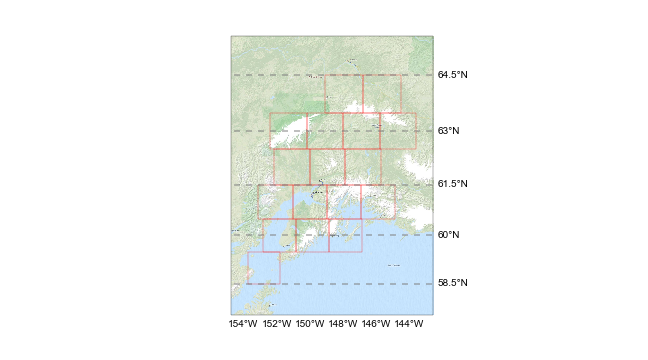
\includegraphics[width=178mm]{figures/westernMap} \centering \caption{Mascons of the western Gulf of Alaska.} \label{fig:wGOA_map}
\end{figure}

\begin{figure}
\noindent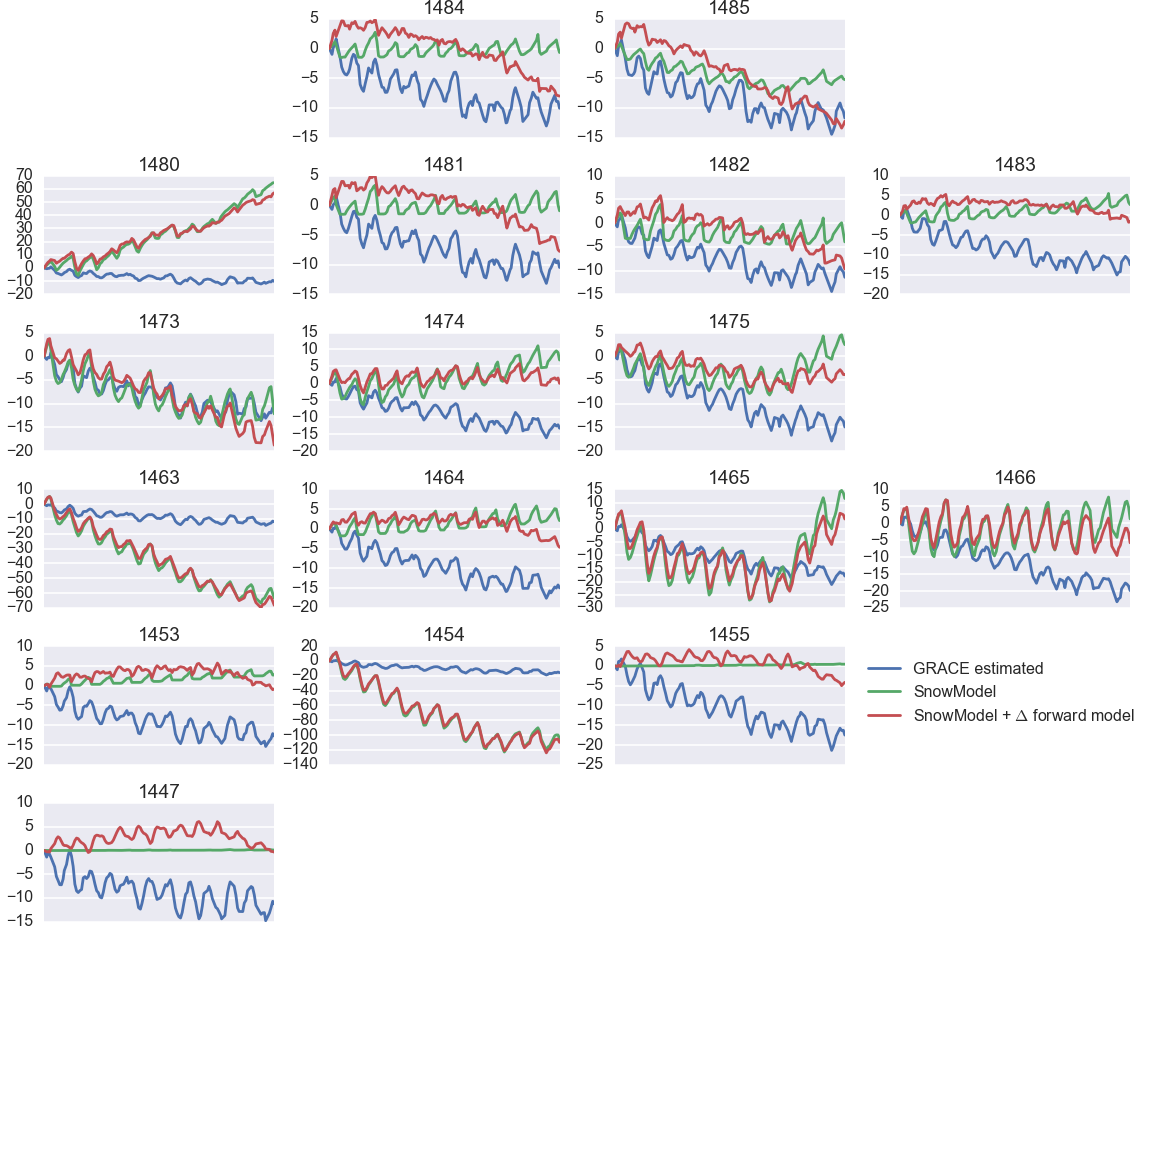
\includegraphics[width=178mm]{figures/westernPlot} \centering \caption{Comparison of GRACE water balances prior to forward modeling \citep{luthcke_antarctica_2013}, (blue); modeled water balances using SnowModel \citep{beamer_high-resolution_2016} (green); and modeled water balance corrected by the forward modeling in this study (red). Subplots are arranged to approximately match the geographic layout of thier respective mascons in Fig. \ref{fig:wGOA_map}} \label{fig:wGOA_plot}
\end{figure}

\begin{figure}
\noindent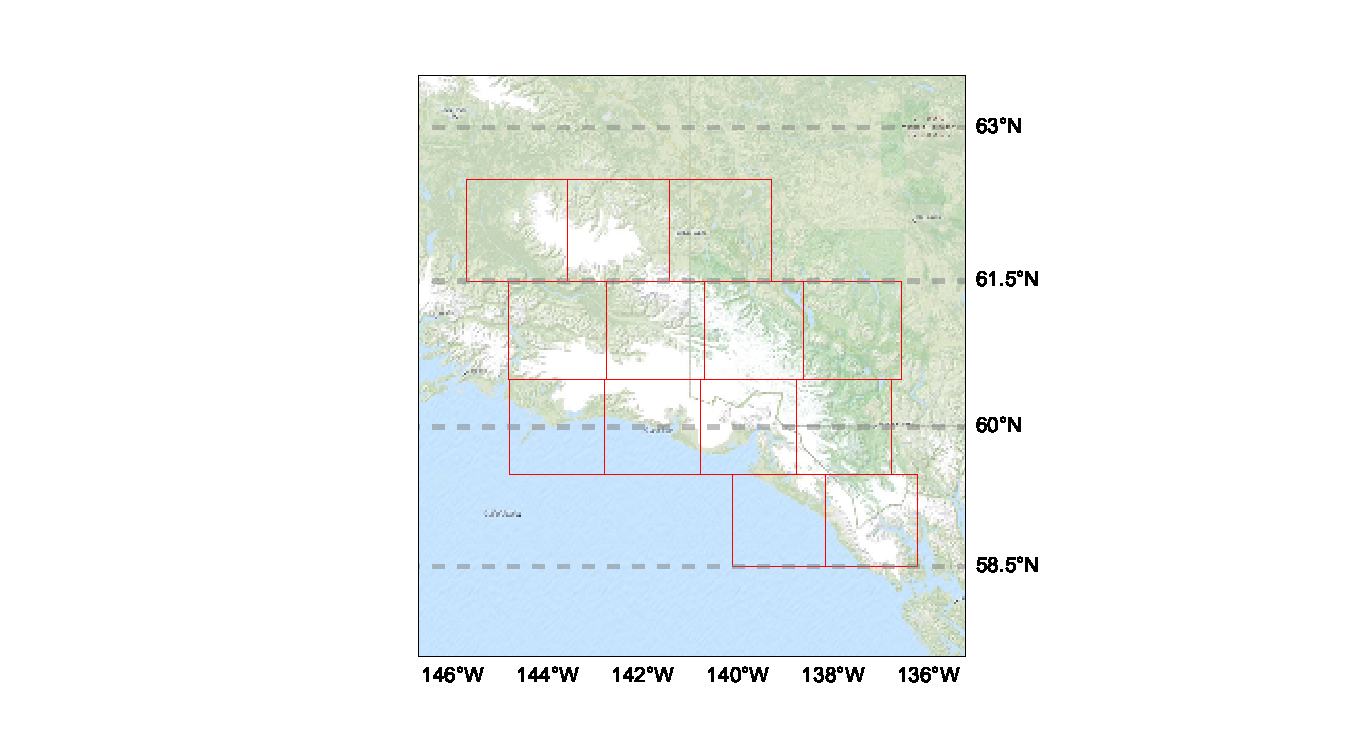
\includegraphics[width=178mm]{figures/easternMap} \centering \caption{Mascons of the western GOA} \label{fig:summer}
\end{figure}

\begin{figure}
\noindent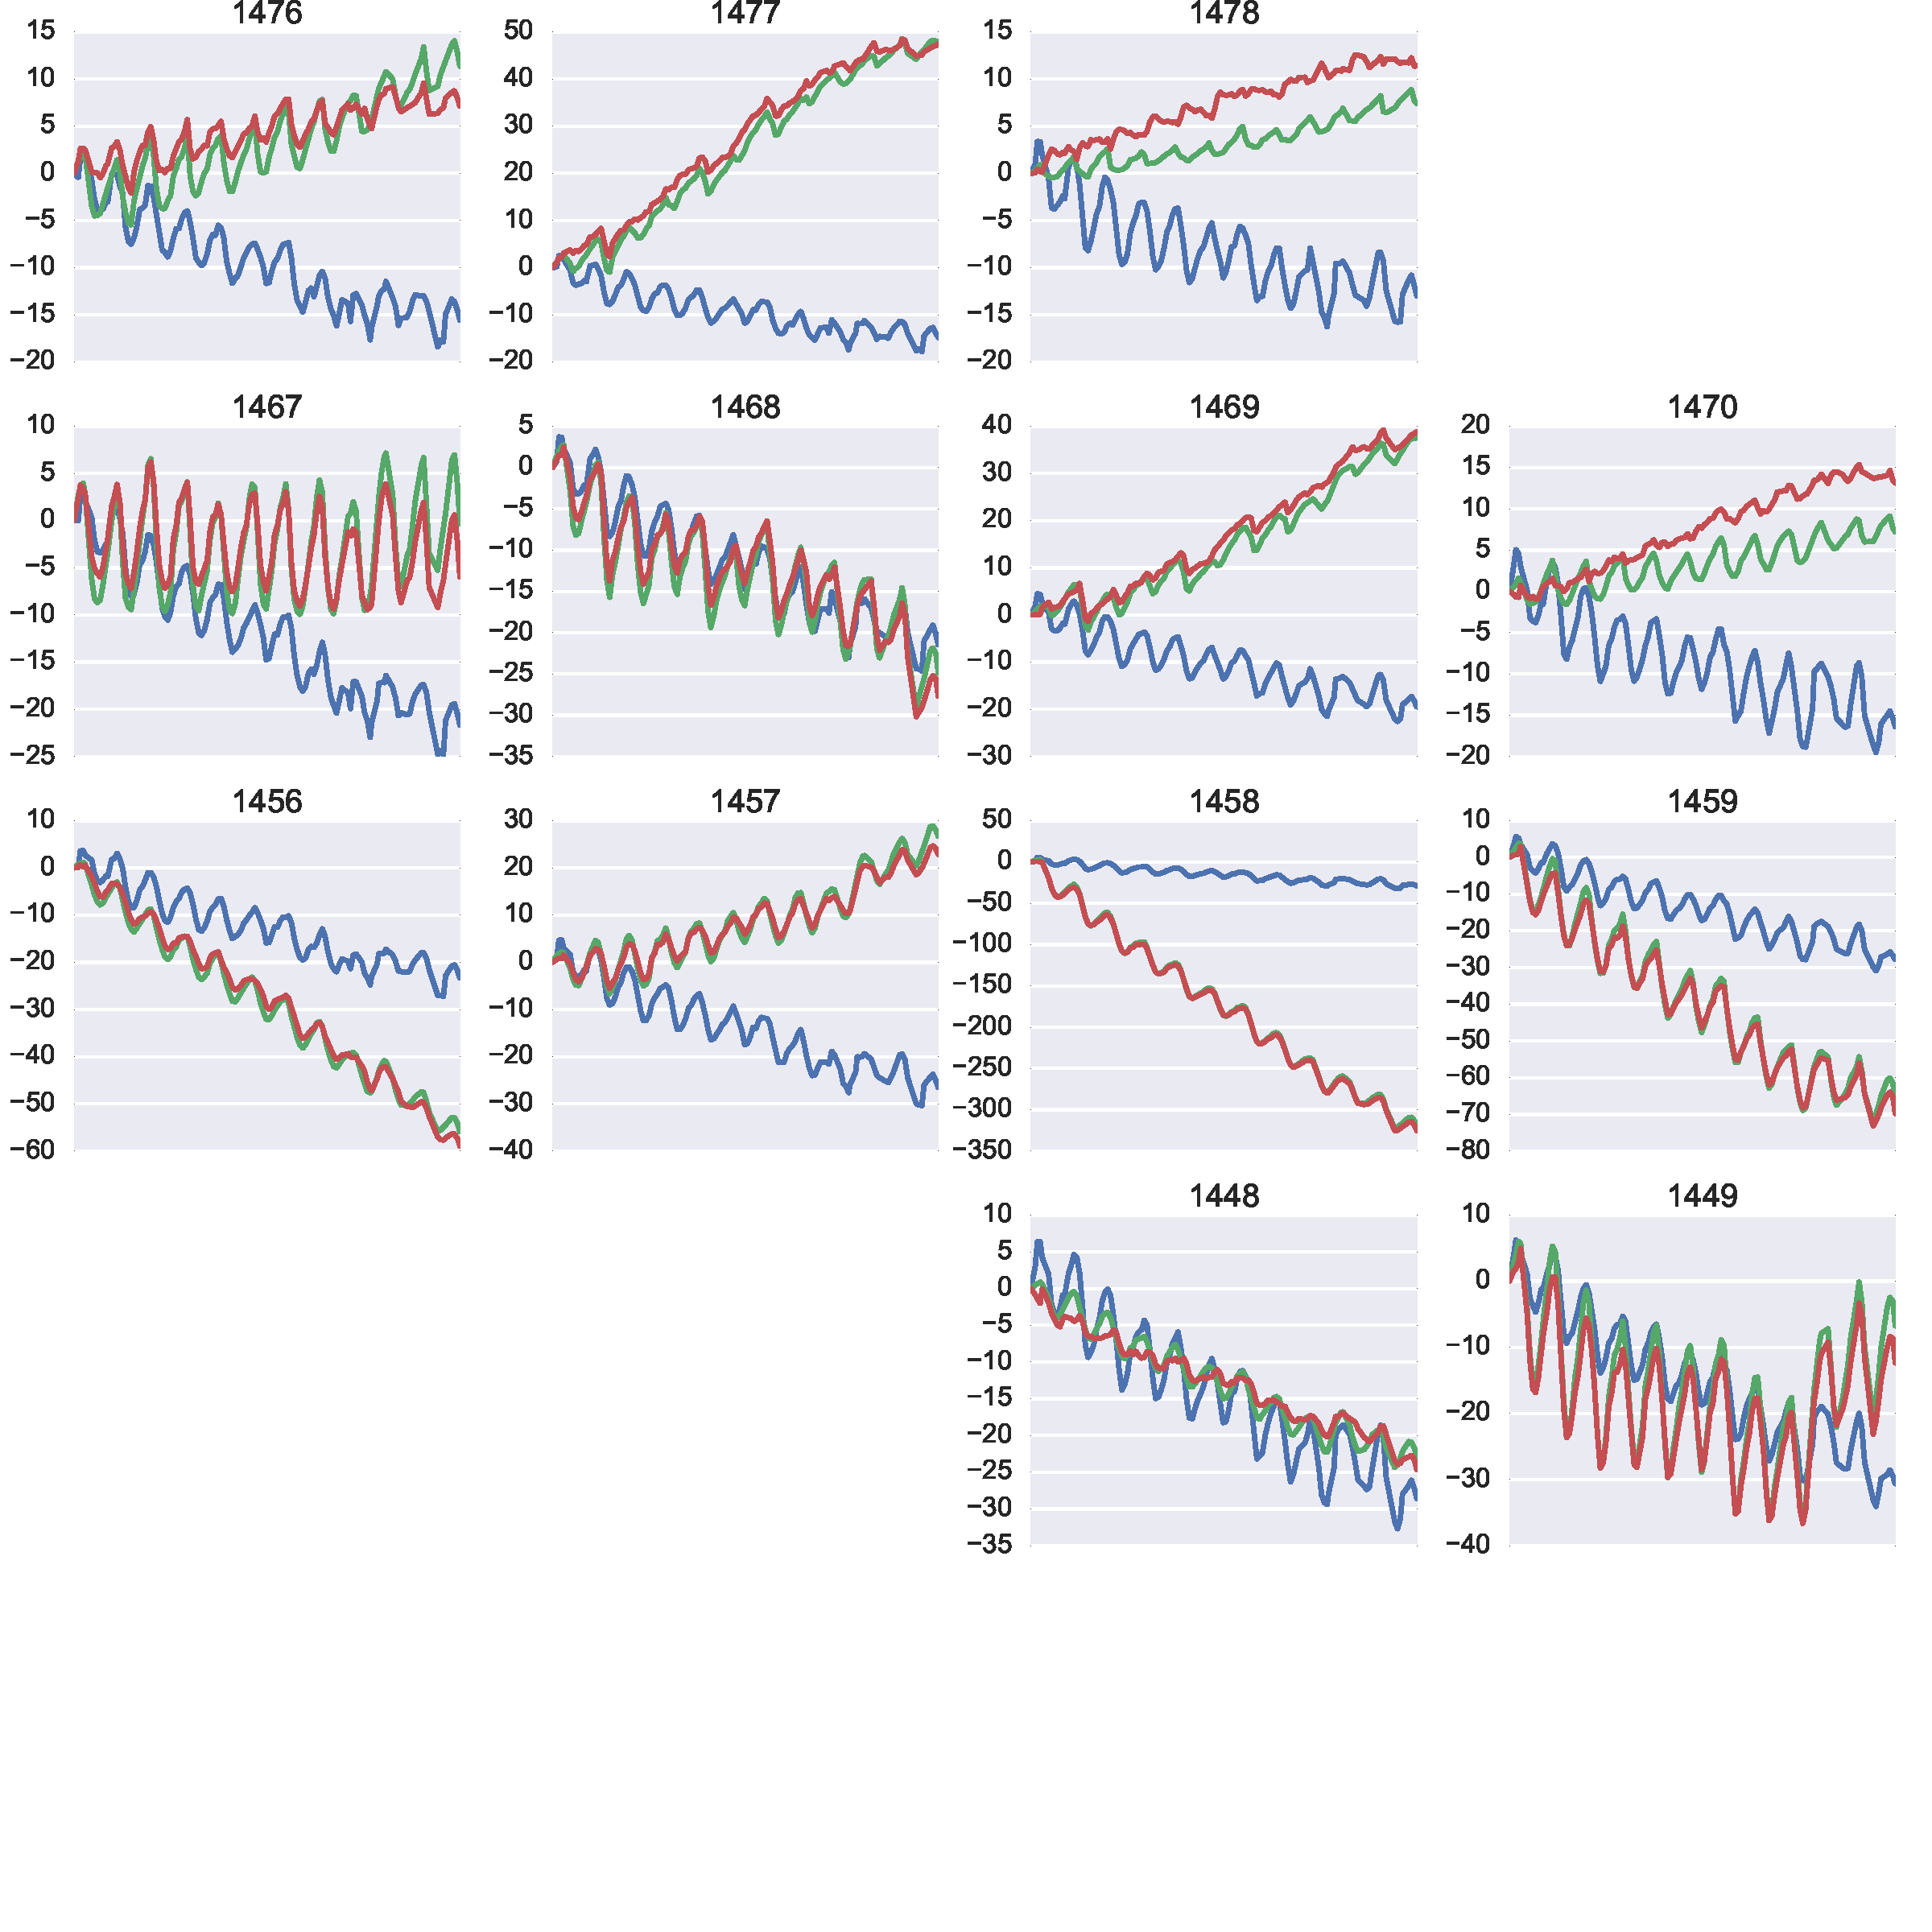
\includegraphics[width=178mm]{figures/easternPlot} \centering \caption{Mascons of the western GOA} \label{fig:summer}
\end{figure}


\begin{figure}
\noindent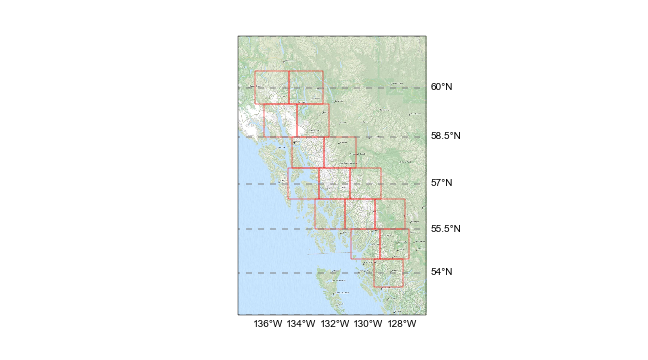
\includegraphics[width=178mm]{figures/southeasternMap} \centering \caption{Mascons of the western GOA} \label{fig:summer}
\end{figure}

\begin{figure}
\noindent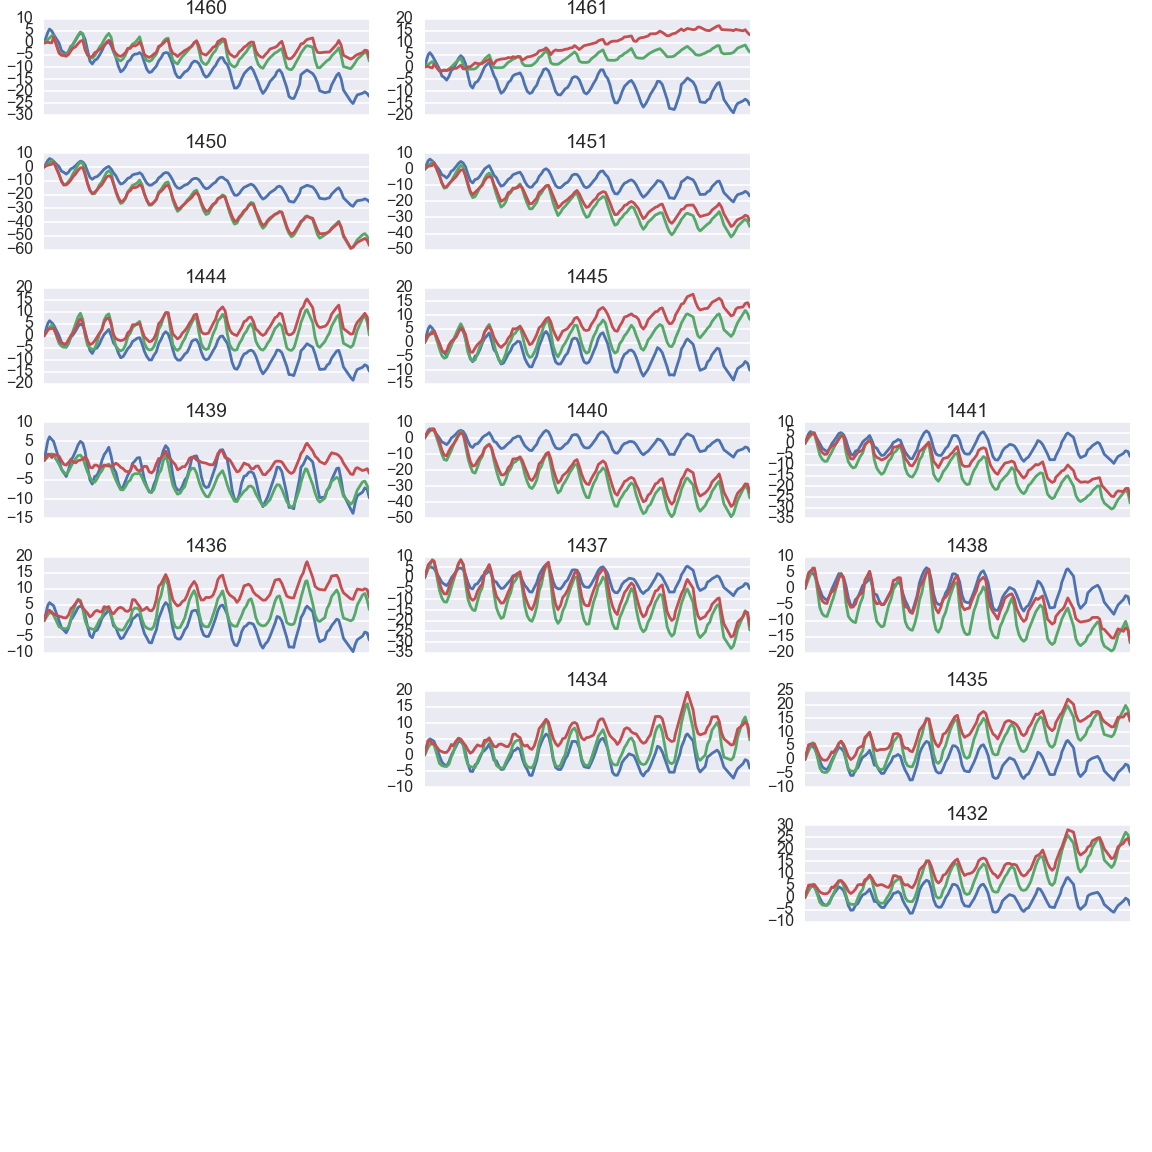
\includegraphics[width=178mm]{figures/southeasternPlot} \centering \caption{Mascons of the western GOA} \label{fig:summer}
\end{figure}

% width = 86 mm
%\begin{figure}[h]
%\includegraphics[width=178mm]{figures/700mbTempDepart_lowres} \centering \caption{Departures in summer (June to August) 700 mb air temperature (mean of NCEP R-2 and ERA-40 reanalysis) from 2004-2010 mean at each of the eight GRACE mascon drainage systems.} \label{fig:upperAir}
%\end{figure}


\end{document}
